\documentclass[aspectratio=169]{beamer}
\usepackage[italian]{babel} 
\usepackage[utf8]{inputenc} 
\usepackage{fourier} 


%Slide colors
\usetheme{Boadilla}
\usecolortheme{beaver}

% Images
\usepackage{graphicx}
\usepackage{caption}
\usepackage{subcaption}
\usepackage{float}
\graphicspath{ {../Images} }

% FlowChart
\usepackage{smartdiagram}

% Stop hyphenation
\usepackage[none]{hyphenat}

% Command to enumerate frames title
\newcommand{\numcirc}[1]{%
	%   \usebeamerfont*{item projected}%
	\large
	\usebeamercolor[bg]{item projected}%
	\begin{pgfpicture}{-1ex}{0ex}{1ex}{2ex}
		\pgfpathcircle{\pgfpoint{0pt}{.75ex}}{1.2ex}
		\pgfusepath{fill}
		\pgftext[base]{\color{fg}#1}
	\end{pgfpicture}%
	\usebeamerfont*{frametitle}%
}


%Header
\title[Tour guidato per bambini ai Musei civici]{\textbf{Manuale per operatori.\\Tour guidato per bambini ai Musei civici.}}
\author{Alice Balestieri}
\date{}

\begin{document}
	
	\begin{frame}
		\maketitle
	\end{frame}
	
	\begin{frame}
		\tableofcontents
	\end{frame}

% Section here	
\section{Schema posizionamento Opere all'interno del Museo.}
	
	\begin{frame}{Schema posizionamento Opere all'interno del Museo}
		\centering {\scalebox{0.67}{\begin{minipage}{\textwidth}
				
					\begin{center}
					\smartdiagramset{set color list={green!60!lime,red!80!black, blue!50!cyan, brown!80, violet!80}, back arrow disabled=true, module minimum width=10cm, module minimum height=1.5cm, module y sep=2.30, arrow line width=0.16cm, text width=8cm}
					\smartdiagram[flow diagram]{Scalone ingresso opera ceramica:\\ \textbf{La Medusa di Ferruccio Mengaroni}, Sala Giovanni Bellini: \\ \textbf{Opere di natura Ecclesiastica e provenienti dalla collezione Rossini},
						Sala delle ceramiche collezione di Domenico Mazza: \\ \textbf{Piatto in ceramica con scoiattolo nero}, Sala arredi e sculture collezione Mosca, Sala natura e inganno}
				\end{center}
				
		\end{minipage}}}
	
	\end{frame}
	
	% Section here
	\section{Che cosa spiegare:}
	
	\begin{frame}{\numcirc{1} Mostrare la Medusa di Ferruccio Mengaroni.}
		\begin{itemize}
			\item 	Mostrare la Medusa di Ferruccio Mengaroni, situata accanto allo scalone d'ingresso ai Musei sulla sinistra, raccontando della maledizione legata all'imponente opera ceramica.\par
			\begin{minipage}{\linewidth}
				\centering
				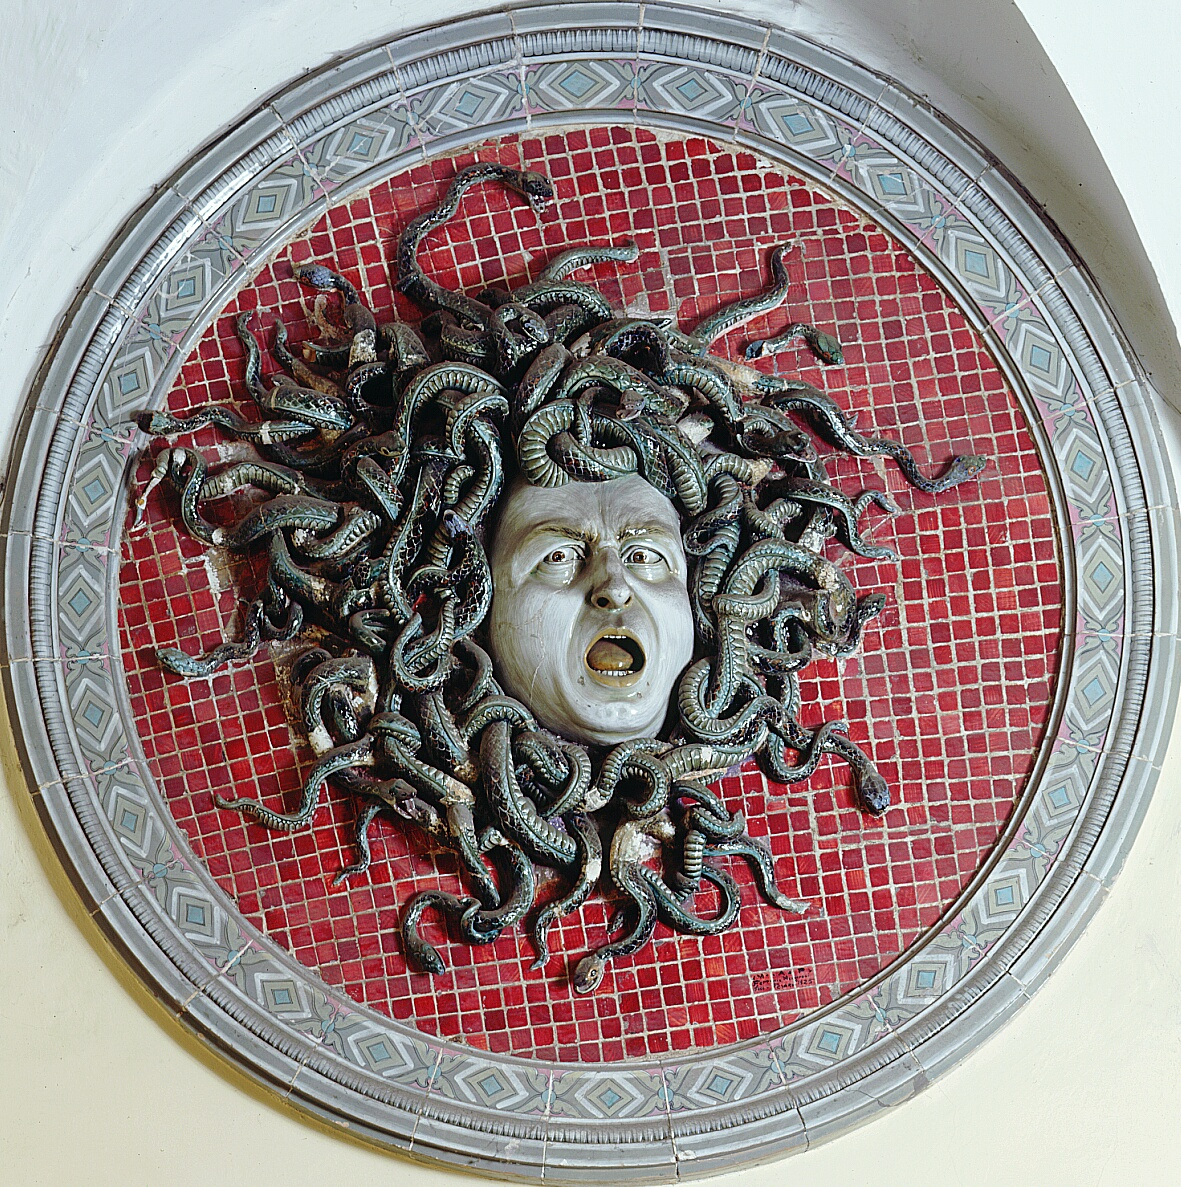
\includegraphics[]{Mengaroni_Ferruccio-Medusa.jpg}
				\captionof{figure}{Mengaroni Ferruccio - Medusa.}
			\end{minipage}
		\end{itemize}
	\end{frame}
	
	
\end{document}